% Paper compiled from RevTeX 4.2 Template (Overleaf)

\documentclass[preprint,
letterpaper,
 amsmath,amssymb,
 aps,
%floatfix,
]{revtex4-2}

\usepackage{graphicx}% Include figure files
\usepackage{dcolumn}% Align table columns on decimal point
\usepackage{bm}% bold math
\usepackage{hyperref}% add hypertext capabilities
\usepackage[mathlines]{lineno}% Enable numbering of text and display math
\usepackage{setspace}
\usepackage{siunitx}
\usepackage{enumitem}
\newcommand{\ts}{\textsuperscript}
\usepackage{amsmath}

\usepackage[utf8]{inputenc}
\usepackage{float}
\newcommand{\iu}{{i\mkern1mu}}
\def\code#1{\texttt{#1}}


\begin{document}
\doublespacing
\title{Gravitational Wave Detection:\\
On the performance of matched filtering and $\chi^2$ consistency testing in the presence of Gaussian noise, non–Gaussianly distributed noise, and transient glitches}
\author{Vinh Nguyen}
\email[Mentored by Dr. Eric Myers – Department of Physics and Astronomy, State University of New York at New Paltz]{}
\affiliation{2020 Pioneer Academics Program \\ Klein Oak High School, Spring, TX 77379}
\date{July 15, 2020}
\begin{abstract}
Lorem ipsum dolor sit amet, consectetur adipiscing elit. Curabitur mattis quam ligula. Suspendisse tempor ante felis, nec tincidunt risus pulvinar sed. Maecenas bibendum imperdiet odio, quis cursus lacus vulputate at. Donec pharetra cursus felis eget ultrices. Phasellus semper, lorem sit amet placerat interdum, ex purus semper nunc, nec accumsan nisl purus quis tellus. Etiam ac ornare augue. Integer ullamcorper malesuada ante, at mattis dui commodo sed. Donec commodo dictum turpis ut suscipit. Pellentesque habitant morbi tristique senectus et netus et malesuada fames ac turpis egestas.
\end{abstract}
\maketitle
\section{Introduction}
Ever since Einstein's first prediction of the existence of gravitational waves in 1915, gravitational wave science and detection have been a leading scientific field of interest. With the first confirmed detection of a binary black hole merger in 2015 (event GW150914), the prospects of gravitational wave science and its applications to other fields such as astronomy and fundamental physics have only become brighter. Gravitational wave detection, however, poses many challenges. This paper explores several challenges in the detection and data analysis of gravitational waves. Specifically, it studies the performance of the optimal matched filter in different noise conditions present in the Virgo and LIGO gravitational wave detectors.

This paper uses LIGO data queried from the Gravitational Wave Open Science Center (GWOSC) is a collaborative effort between the LIGO Laboratory, the LIGO Scientific Collaboration and the Virgo Collaboration to provide the public with gravitational wave data from the two LIGO facilities (Hanford, WA and Livingston, LA) as well the Virgo Observatory in Cascina, Italy

\section{Background}
\subsection{Gravitational waves and the Laser Interferometer Gravitational-Wave Observatory (LIGO)}
In 1915, Einstein first published his theory of general relativity, describing space and time as one four-dimensional concept called \textit{``space-time''} \cite{maggiore_2008}, In this theory, he describes the force of gravity not as an inherent property that a massive body possesses, but rather as a byproduct of curved space-time. To put this more simply, we can say that a body with mass warps space-time, thereby creating a gravitational field surrounding it, affecting other bodies \cite{carlip}. To understand this idea, we can make use of an analogy: suppose that the fabric of space-time is a rubber sheet, and that any object with mass on it warps the surrounding area (FIG. 1.), hence creating a gravitational field. It follows from Einstein's Theory of Relativity that rapid changes in the curvature of space-time would produce ripples, called \textit{gravitational waves} (abbreviated as GW), that propagate outward at the speed of light  \cite{JSTORLIGO}.

\begin{figure}[t]
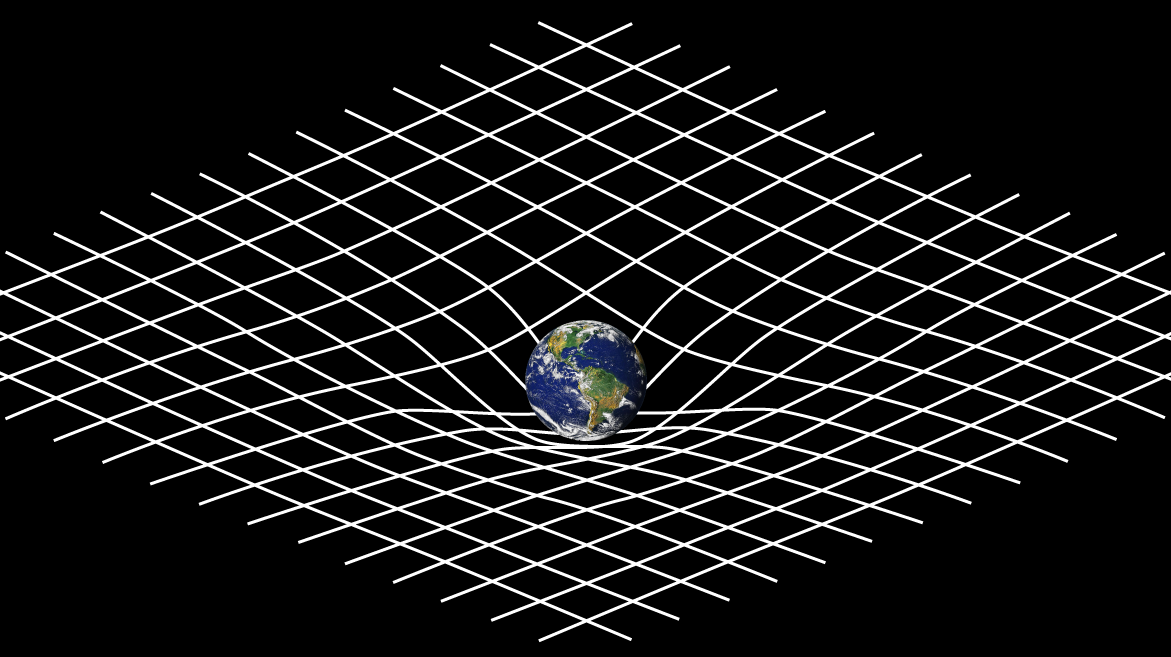
\includegraphics[width=8cm]{genral.png}
\caption{This figure shows a simplified analogy for Einstein's idea of space-time – which cannot be fully illustrated by a 2D picture. Adapted from \cite{mattson}.}
\centering
\end{figure}

LIGO (short for Laser Interferometer Gravitational-wave Observatory) is an NSF-funded, large scale scientific collaboration between the California Institute of Technology and the Massachusetts Institute of Technology designed to detect gravitational waves. As of June 2020, LIGO has two site locations – one in Hanford, Washington and the other in Livingston, Louisiana. Another important scientific collaboration is the Virgo project. The Virgo project is a European collaboration for gravitational wave detection funded by the French Centre National de Recherche Scientifique (CNRS), the Italian Istituto Nazionale della Fisica Nucleare (INFN), the Dutch Nikhef in addition to the Polish and Hungarian institutes \cite{collaboration2019open}. Virgo has one detector located in Cascina, Italy. The two LIGO sites as well as the Virgo site in Italy each employs a type of detector called the Michelson Fabry-Perot Interferometer (interferometer for short) \cite{creighton_anderson_2011}. Virgo/LIGO's interferometers function by using four test masses (in this case, mirrors) in an L-shaped configuration, hung by wires near the ends and the vertex of the `L' as shown in FIG. 2. The test masses are configured so that the length $L_1 \approx L_2 = L$ (note that at the frequency of around $1$ Hz, the test masses can move freely horizontally) \cite{JSTORLIGO}. 

\begin{figure}
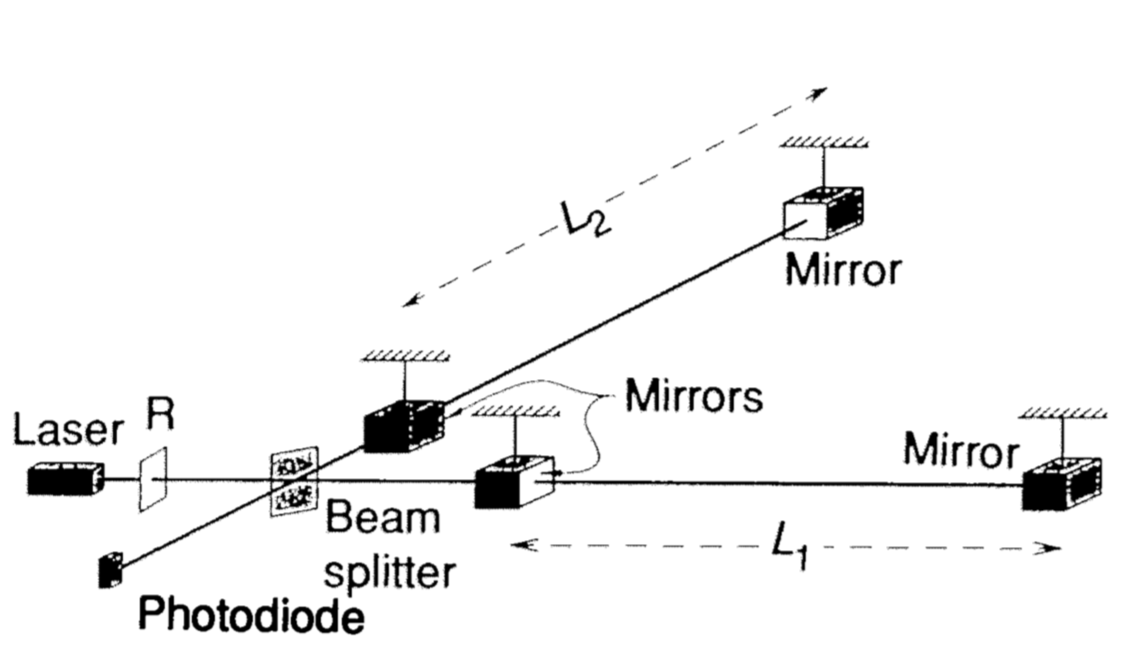
\includegraphics[scale = .4]{Interferometer.png}
\caption{A simplified diagram of the Michelson Fabry-Perot Interferometer. Adapted from \cite{JSTORLIGO}.}
\centering
\end{figure} 
If there is a gravitational wave passing in between the test masses, the space between them will be stretched and compressed, squeezing one arm while stretching the other such that we can calculate the value of the arm length difference $\Delta L = L_1 - L_2$ \cite{teacherintro}. To measure this quantity $\Delta L$, the device uses a technique called laser interferometry \cite{LIGOArxiv}. Specifically, a powerful laser beam is shined at the beam splitter, thereby splitting the beam in half along the two arms. These beams then each enter a Fabry-Perot cavity where they are reflected back and forth between the mirrors, building up the laser light within the interferometer and increasing the distance travelled by the beam \cite{fabry} – increasing the interferometer's sensitivity. As the laser beams in the two arms exit the Fabry-Perot cavity and return to the beam splitter, the splitter recombines the two half-beams and gives off a portion of the combined beam to a photodiode – hence allowing scientists to analyze the interference patterns of the waves using optics principles, and thus determine the quantity $\Delta L$. 

For gravitational waves passing through the test masses, the fractional difference in arm length $\frac{\Delta L}{L}$ is the strain $h$ (a quantity that measure the `strength' of gravitational waves) of the waves. Mathematically, the strain $h(t) = \frac{\Delta L(t)}{L}$ can also be expressed as a linear combination of its cross and plus polarizations, as follows \cite{JSTORLIGO}:
\begin{equation}
h(t) = F_\times h_\times (t) + F_+ h_+ (t)
\end{equation}

\subsection{LIGO Data Analysis and Conventions}
\subsubsection{The Fourier Transform}
The signal from Virgo/LIGO is recorded as a function of time. However, to process this signal, we must usually transform the signal from its original time-domain into its frequency-domain through the use of a mathematical tool called the \textit{Fourier Transform}. In simplest terms, the Fourier Transform decomposes a function into its frequency content. Given a \textit{continuous} time-series function $F(t)$, its frequency-domain representation $\widetilde{F}(f)$ is given by \cite{dsptextbook}:
\begin{equation}
\widetilde{F}(f) = \int_{-\infty}^{\infty}F(t)e^{-2\pi\iu ft} dt
\end{equation}

Notice that $\widetilde{F}(f)$ is a complex-valued function whose magnitude represents the frequency amplitude and whose argument represents the phase offset. Similarly, a frequency-domain continuous function $\widetilde{F}(f)$ can also be transformed back into its time-domain representation using an \textit{inverse Fourier Transform}. Given $\widetilde{F}(f)$, $F(t)$ can be calculated by the equation:
\begin{equation}
F(t) = \int_{-\infty}^{\infty}\widetilde{F}(f)e^{2\pi\iu ft} df
\end{equation}

Unfortunately, LIGO signal is not a continuous function in the time-domain, thus we have to \textit{discretize} our formulas for both the continuous forward and the continuous inverse Fourier Transforms \cite{dsptextbook}. Given a time-domain signal \textit{sequence} $f[n]$, the frequency-domain representation $\widetilde{f}[n]$ can be obtained using the discrete Fourier Transform (DFT) as follows\cite{roberts_2020}:
\begin{equation}
\widetilde{f}[n]=\sum _{n=0}^{N-1}f[n]\cdot e^{-{\frac {2\pi}{N}\iu kn}}
\end{equation}

The time-domain sequence $f[n]$ can be then obtained from the frequency-domain sequence $\widetilde{f}[n]$ through the inverse discrete Fourier transform (with a normalization factor) as such \cite{roberts_2020}:
\begin{equation}
f[n]=\frac{1}{N}\sum _{n=0}^{N-1}\widetilde{f}[n]\cdot e^{{\frac {2\pi}{N}\iu kn}}
\end{equation}

Since we are working with discrete-valued sequences, performing a DFT would give rise to spectral leakages. Thus, to minimize this, we always apply a windowing function to data in this paper whenever the use of the DFT is required (note that windowing does not decrease spectral leakage, but rather re-distributes the leakage effect so that it causes the least harm). In this paper, I also use a computer algorithm that implements the discrete Fourier Transform called the Fast Fourier Transform (FFT) which is implemented within the Python PyCBC library \cite{numpy}.

\subsubsection{Noise characteristics}
Being able to reach a strain sensitivity of $10^{-23}/\sqrt{\text{Hz}}$ \cite{sensitivity} means Virgo/LIGO's interferometers are extremely sensitive to any changes in the arm lengths – which can be caused by distorted space-time due to gravitational waves, or by vibrations that move the test masses. Thus, recorded signal $s(t)$ includes not only gravitational waves, but also unwanted vibrations from other sources as well \cite{ultimate}. Any unwanted noise, even on the smallest of scales, can still significantly interfere with data recorded by Virgo/LIGO's interferometers. Virgo/LIGO noise comes from many sources, but some examples include seismic noise due to motions of the Earth's surface, thermal noise at the molecular level affecting the test masses, and quantum shot noise at high frequencies caused by the quantum nature of light \cite{blair_howell_ju_zhao_2012}.

In order to extract buried gravitational wave signals from noise, we must first understand the statistical properties of the noise. Noise is said to be stationary if its statistical properties do not significantly change over time. Another important noise characteristic is its Gaussianity. Given \textit{`Gaussian'} noise with a time-series function $n(t)$, both the real and imaginary components of its Fourier Transform $\widetilde{n}(f)$ follow the normal distribution \cite{yamamoto}; that is, $\Re[\widetilde{n}(f)]$ and  $\Im{[\widetilde{n}(f)]}$ have a probability density function (PDF) of:
\begin{equation}
    p(x) = \frac{1}{\sigma\sqrt{2\pi}}\exp{\left(-\frac{1}{2}\frac{(x-\mu)^2}{\sigma^2}\right)}
\end{equation}
where $\sigma^2$ is the sample variance and the mean $\mu = 0$. By the Central Limit Theorem in statistics, a set of random noise sample naturally tends to the Gaussian distribution if sufficiently large data samples were taken \cite{jaranowski2007gravitationalwave}. Nonetheless, real Virgo/LIGO noise can still deviate from normality due to abrupt noise sources such as short-duration transient noise of, sometimes, unknown origins called glitches \cite{ultimate}. Noise can also follow a variety of different probability density distributions such as the Poisson distribution and the Laplace distribution. Although it is not common in real-life Virgo/LIGO operations that these noise models are present, this paper still considers the case of Laplacian noise for theoretical analysis purposes. It is worth pointing out that over short time intervals, however, Virgo/LIGO noise can still be reasonably approximated to be Gaussian and stationary \cite{collaboration2019open}.

\subsubsection{Matched filtering}
The primary goal of Virgo/LIGO data analysis is to determine if there is gravitational wave signal buried in the noise. There are many ways that this can be accomplished; however, the most efficient and effective method is called \textit{matched filtering}, especially in cases where noise is both Gaussian and stationary \cite{helstrom_1975}. Matched filtering allows the recorded data stream to be searched for the presence of a known gravitational wave template with varying arrival time and phase offset \cite{surf}.  A matched filter requires three components: the recorded data stream $s(t)$, the \textit{power spectral density (PSD)} function $S_n(t)$ of the noise, and a known waveform template $h(t)$ of the gravitational wave. Given these quantities, the complex-valued output of the matched filter at time $t=t_0$ can be computed as follows \cite{findchirp}:
\begin{equation}
    z(t_0) = 4\int_0^\infty\frac{\widetilde{s}(f)\widetilde{h}^*(f)}{S_n(f)}e^{2\pi\iu ft_0}df
\end{equation}
where $\widetilde{h}^*(f)$ denotes the complex conjugate of the Fourier Transform of the template strain $h(t)$. Notice that the existence of $S_n(f)$ essentially down-weighs the frequencies where the noise is loud and does the opposite where the noise is weak \cite{ultimate}. Given the complex matched filter output $z(t)$, we can compute a test statistic value $\rho$ called the \textit{signal-to-noise ratio} as follows \cite{findchirp}: 
\begin{equation}
   \rho (t) = \frac{|z(t)|}{\sigma}
\end{equation}
where $\sigma$ is a normalization factor is computed from \cite{findchirp}
\begin{equation}
   \sigma^2 =  4\int_0^\infty\frac{|\widetilde{h}(f)|^2}{S_n(f)}df
\end{equation}

 Notice that here, the template waveform is computed using a set of parameters of the astrophysical source (e.g.\ the total mass, the spins, the initial frequency, etc of a binary inspiral). The goal of a matched filter search process is to see which template would give the highest SNR $\rho (t)$, and thus is mostly likely to be the strain signal in the data stream. 
 
In the presence of non-Gaussian and/or non-stationary noise and/or glitches, the matched filter does not perform as well as expected since the filter itself is derived from Gaussian and stationary noise. A detailed mathematical derivation of the matched filter from a stationary, Gaussian noise model can be found in \textit{Brown (2007)} \cite{brown2007searching}.


There are several ways of incorporating the matched filter into a computer program that analyzes LIGO's signal. In this paper, I only make use of the matched filtering algorithm implemented in the open-source Python software package PyCBC \cite{pycbc}. This algorithm is based on the FINDCHIRP algorithm presented above and in \cite{findchirp}.


\section{Methodology}

This paper sought to evaluate the performance of the matched filtering algorithm implemented in the PyCBC software package. The evaluation focused on 3 aspects of the signal extraction output:
\begin{itemize}
    \item Performance in the presence of perfectly Gaussian noise with $\mu = 0$  and $\sigma = 1$ scaled down by a factor of $10^{-21}$.
    \item Performance in the presence of non-Gaussian noise – in this case, Laplacian noise with location $\mu = 0$ and scale parameter $b = 1,2,3$. Laplacian noise with  $\mu = 0$ and varying $b$ was chosen for the purposes of this study due to its symmetric nature (similar to Gaussian noise) and varying levels of kurtosis. The higher the scale value $b$, the heavier the Laplacian noise distribution will be at the tails (note that heavier tails correspond to higher kurtoses). These Laplace distributed noise models were all scaled down by a factor of $10^{-21}$. An illustration of these distributions are shown in FIG. 3.
    \item Performance in the presence of transient glitches. In this paper, I used five samples of known Virgo/LIGO glitches with two \textit{`Extremely Loud'} glitches, one \textit{Scattered Light} glitch, one \textit{Whistle} glitch, and one \textit{Power Line} glitch.

\end{itemize}

In the case of glitches, I employed 50 seconds around the time of peak amplitude of the glitches. A full catalog documentation of known Virgo/LIGO transient glitches was provided by Michael Zevin (PhD Candidate at Northwestern University) and the GravitySpy team \cite{gravityspy}.  The glitch samples chosen for this study are as follows:

\begin{figure}[t]
\caption{The different probability density functions $f_X(x)$ are shown below. Since $\int_{-\infty}^\infty f_X(x)dx = 1$, the lower the  functions' maximums are, the heavier their tails must be, leading to higher kurtoses.}
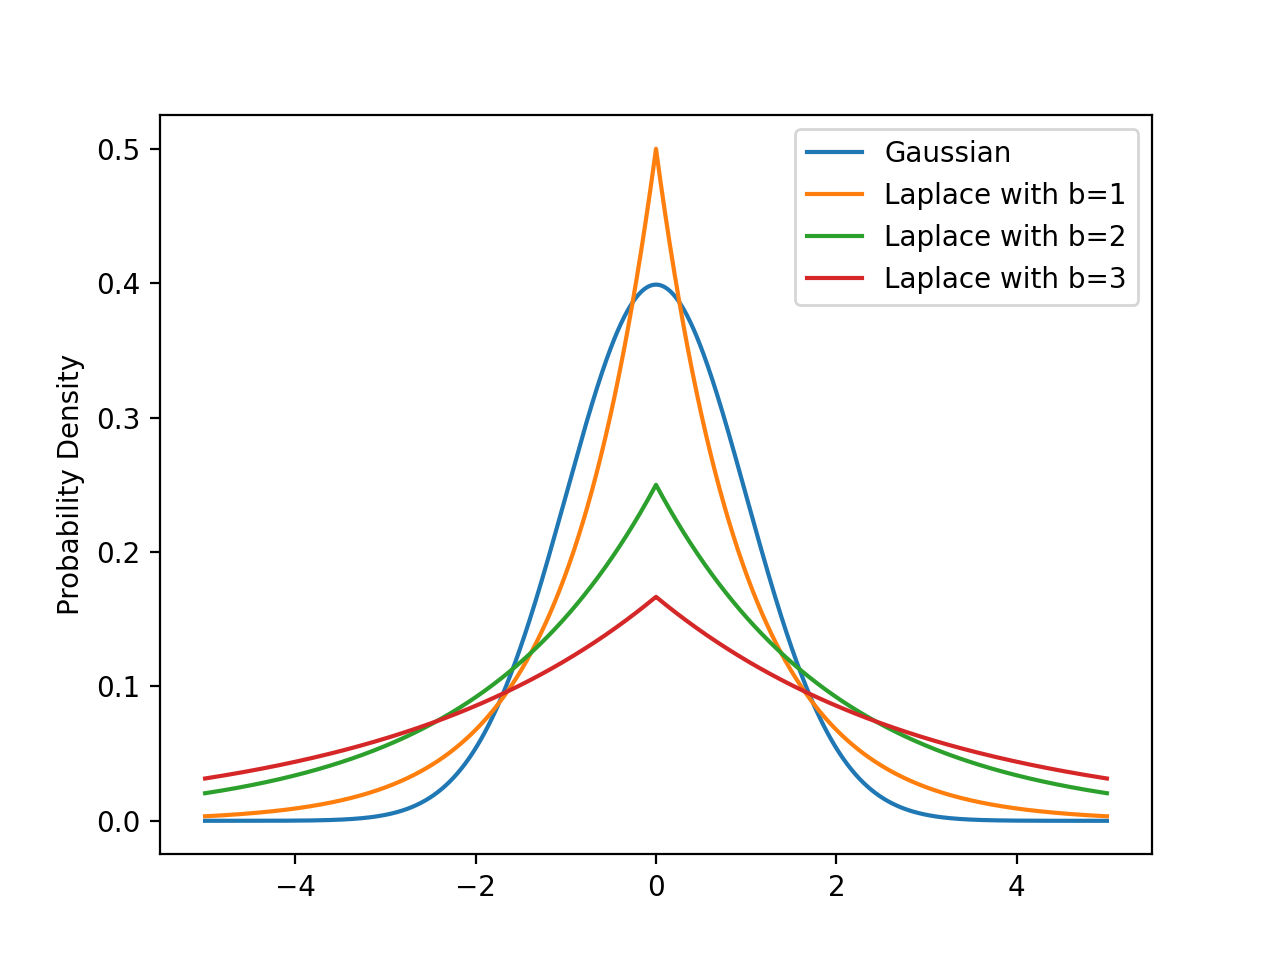
\includegraphics[scale = .54]{pdf graphs.png}
\centering
\end{figure}


\begin{itemize}
\item Glitch 1: An \textit{`Extremely Loud'} glitch found at the Virgo detector on August 2$^{\text{nd}}$, 2017, 17:04:11 UTC (GPS time 1185728669).

\item Glitch 2: Another \textit{`Extremely Loud'} glitch, also found at the Virgo detector but on August 19$^{\text{nd}}$, 2017, 05:41:24 UTC (GPS time 1187156502).

\item Glitch 3: A \textit{Scattered Light} glitch found at the Livingston detector on December 3$^{\text{rd}}$, 2016, 04:17:11 UTC (GPS time 1164773848).

\item Glitch 4: A \textit{Power Line glitch} found at the Hanford detector on August 15$^{\text{th}}$, 2017, 01:59:25 UTC (GPS time 1186797583).

\item Glitch 5: A \textit{Whistle} glitch found at the Livingston detector on April 23, 2017, 03:08:21 UTC (GPS time 1176952119).
\end{itemize}

For visualization purposes, strain time-series data of the glitches and their Q-transformed spectrograms are shown from FIG. 4. to FIG. 8.
\begin{figure}[t]
\caption{The top figure shows the strain time-series of 50 seconds around Glitch 1. The bottom figure shows a Q-transformed spectrogram around Glitch 1. (Data queried from \cite{collaboration2019open})}
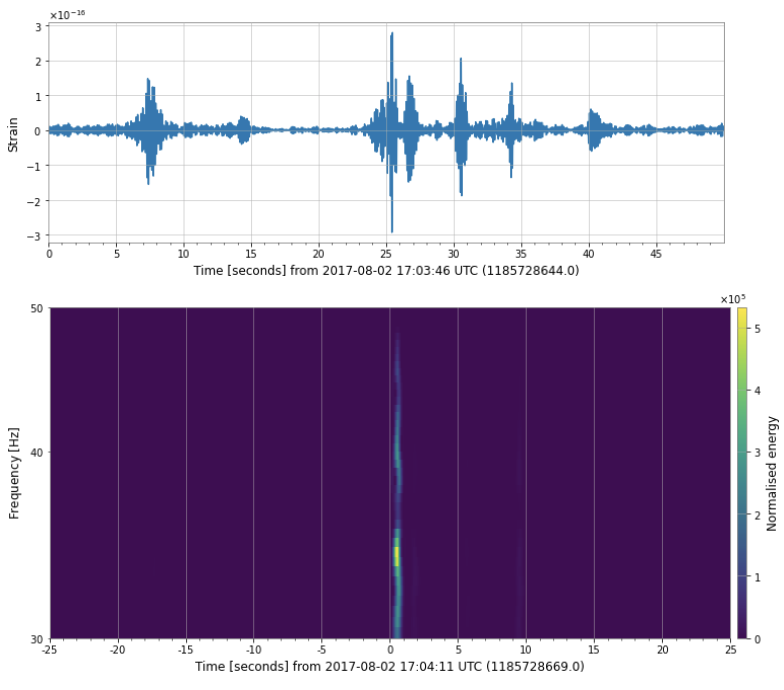
\includegraphics[scale = .6]{loud 69 graphics.png}
\centering
\end{figure} 
\begin{figure}[t]
\caption{The top figure shows the strain time-series of 50 seconds around Glitch 2. The bottom figure shows a Q-transformed spectrogram around Glitch 2. (Data queried from \cite{collaboration2019open})}
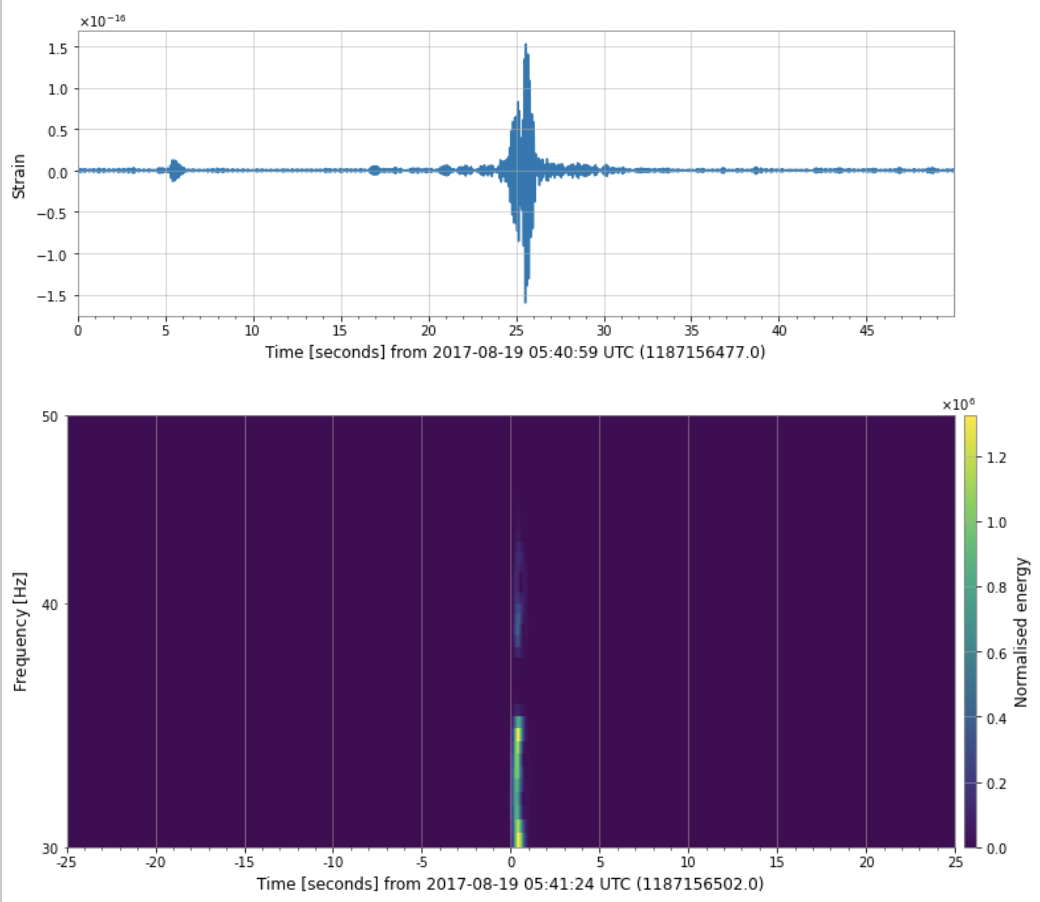
\includegraphics[scale = .45]{loud 02 graphics.png}
\centering
\end{figure} 
\begin{figure}[t]
\caption{The top figure shows the strain time-series of 50 seconds around Glitch 3. The bottom figure shows a Q-transformed spectrogram around Glitch 3. (Data queried from \cite{collaboration2019open})}
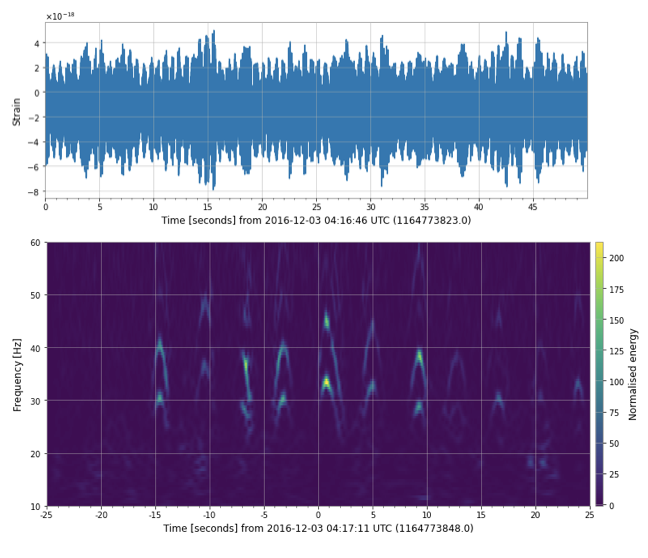
\includegraphics[scale = .75]{Scattered Light Graphics.png}
\centering
\end{figure} 
\begin{figure}[t]
\caption{The top figure shows the strain time-series of 50 seconds around Glitch 4. The bottom figure shows a Q-transformed spectrogram around Glitch 4. (Data queried from \cite{collaboration2019open})}
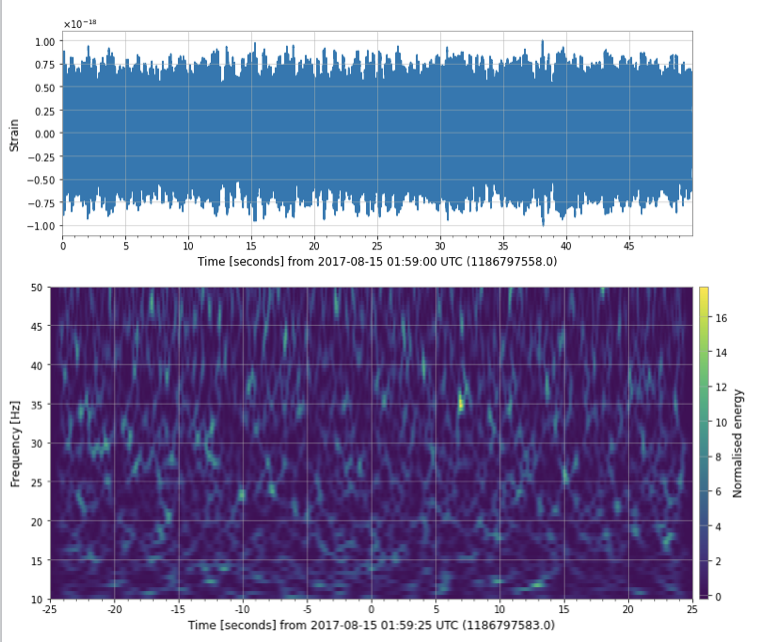
\includegraphics[scale = .6]{power line graphics.png}
\centering
\end{figure} 
\begin{figure}[t]
\caption{The top figure shows the strain time-series of 50 seconds around Glitch 5. The bottom figure shows a Q-transformed spectrogram around Glitch 5. (Data queried from \cite{collaboration2019open})}
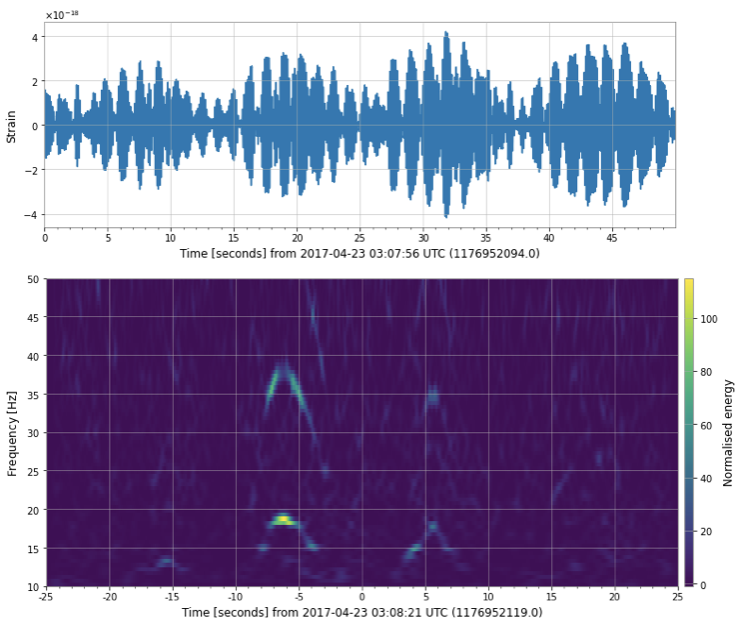
\includegraphics[scale = .65]{whistle graphics.png}
\centering
\end{figure} 

The performance evaluation followed a general method: 

First, I created a time-series template using the post-Newtonian approximation method (a method of approximating Einstein's field equations). The time-series template generation was done using PyCBC's \code{get\_td\_waveform} method; I also only used the plus polarization of the template waveform since this paper studies only the performance of signal extraction algorithms, not the waveforms themselves. 

In this paper, I made use of 3 templates of binary black hole inspirals using the `IMRPhenomD' model as the approximant. The sampling rate for this template, and all subsequent time-series data described in this paper is $4096$ Hz – down-samploed from LIGO's original $16384$ Hz sampling rate. The inspiral parameters for the 3 templates are as follows:
\begin{enumerate}
    \item Two black holes with masses 30 $M$\textsubscript{\(\odot\)} and 23 $M$\textsubscript{\(\odot\)} at an effective distance of 500 Mpc and initial frequency of 14 Hz.
    \item Two black holes both of masses 7 $M$\textsubscript{\(\odot\)}  at an effective distance of 500 Mpc and initial frequency of 40 Hz.
\end{enumerate}

I then proceeded to zero-pad the templates so that their lengths match the length of the 50-second stretch of noise. Afterwards, I `rolled' the templates so that they start at time $t=35$s in the 50-second stretch of data. In the case of Gaussian noise, the pure noise was generated via the Python NumPy package's \code{random.normal} method then scaled down both by a factor of $10^{-21}$ \cite{numpy}. In the case of Laplacian noise, the \code{random.laplace} method was used. It was then scaled down accordingly similar to the Gaussian case. As for the 5 samples of glitches, raw LIGO data of 25 seconds before and after the glitches' time of peak amplitude was queried directly from GWOSC (the code
for this can be accessed at \footnote{V.Nguyen, Google Colab notebook for signal matched filtering and chi-squared consistency testing, \href{https://colab.research.google.com/drive/10q3SdhNjWyoZaVPdLqyoCEsSovplvMrK?authuser=2#scrollTo=7cafQoPiH5Sy}{(2020)}. URL: \url{https://colab.research.google.com/drive/10q3SdhNjWyoZaVPdLqyoCEsSovplvMrK?authuser=2#scrollTo=7cafQoPiH5Sy}}) to be used as the noise (with glitch). Note that these samples of glitches also contain background noise that may or may not be Gaussian and stationary in addition to the glitches themselves. Removing background noise from these samples and extracting these glitches require complex methods that were not attainable within the time frame of the writing of this paper. 

Afterwards, I estimated the PSD of the data. Then, I applied the PyCBC matched filtering algorithm using the \code{matched\_filter} method. The python script implementation of these algorithms can be found at \url{https://tinyurl.com/yaedmpsx}. The signal-to-noise ratio (SNR) $\rho (t)$ computed from the matched filtering algorithm was then cropped by 10 seconds on both ends. The reason for this is that running the matched filter on a data segment of finite length using an estimated PSD gives rise to `edge effects'. In simplest terms, these `edge effects' give extremely high, false SNR peaks near the edges that can be mistaken for gravitational wave signal. Using this final cropped SNR $\rho(t)$, I could then analyze it to evaluate the search's performance.

\section{Results and Data Analysis}
The time-series template waveforms described in \textit{Section IV} are shown in FIG. 9. As seen, these templates are of different lengths, but all less than the 50 seconds duration. Since these templates are all zero-padded and rolled so that they start at time $t=35$s before being injected into the 50 seconds stretch of pure noise (and glitches in that case), the peak-SNR after applying a matched filter is expected to be at time $t=35$s.

\begin{figure}[t]
\caption{This figure at the top shows the template waveform strain time-series of a binary black hole merger with masses 30 $M$\textsubscript{\(\odot\)} and 23 $M$\textsubscript{\(\odot\)} (Template 1). The figure at the bottom shows the template waveform strain time-series of a binary black hole merger with both black holes of mass 7 $M$\textsubscript{\(\odot\)} (Template 2). These waveforms were generated with PyCBC \cite{pycbc}.}
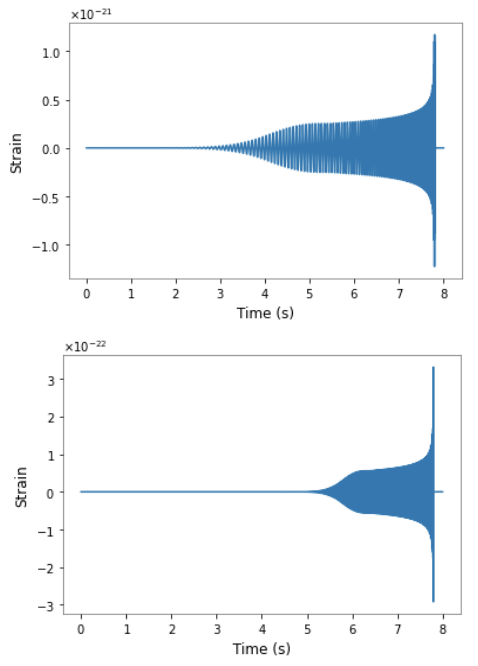
\includegraphics[scale = 1]{templates.png}
\centering
\end{figure} 

The PyCBC matched filtering algorithm yielded reasonable results. Figures 9 to 13 show the SNR as a function of time of the different combinations of noise / glitch and templates recovered.

\begin{figure}[t]
\caption{This figure shows the resulting cropped SNR $\rho(t)$ after a matched filter was applied to recover Template 1 from perfectly Gaussian noise scaled down by a factor of $10^{-21}$. A signal peak was detected at time $t = 35.0$s with SNR $\rho = 20.0$}
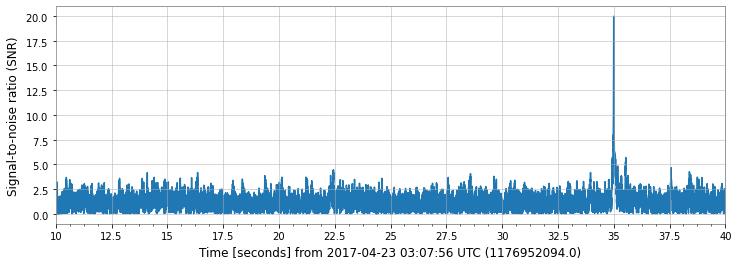
\includegraphics[scale = .33]{gaussian -21 template 1.png}
\centering
\end{figure} 

\begin{figure}[h!]
\caption{This figure shows the resulting cropped SNR $\rho(t)$ after a matched filter was applied to recover Template 1 from perfectly Laplacian noise with $b=1$, scaled down by a factor of $10^{-21}$. A signal peak was detected at time $t = 35.0$s with SNR $\rho = 12.6$.}
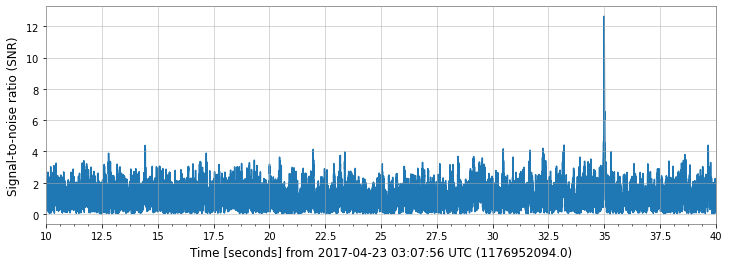
\includegraphics[scale = .33]{laplacian b=1 template 1.png}
\centering
\end{figure} 
It can be seen from FIG. 10. and FIG. 11. that there are clear, thin, and distinct SNR peaks at time $t = 35.0$s. The peak SNR's of these two cases, though, are of different values. In the case of Gaussian noise, the SNR is 20.0, while it is only 12.6 in the case of Laplacian noise with $b=1$. Furthermore, it can also be seen that the SNR `noise-floor' in FIG. 10. is similar to that in FIG. 11. Specifically in both cases, the SNR `noise-floor' varies about $\rho = 3.75$. 

\begin{figure}[t]
\caption{This figure shows the resulting cropped SNR $\rho(t)$ after a matched filter was applied to recover Template 1 from perfectly Laplacian noise with $b=2$, scaled down by a factor of $10^{-21}$. A signal peak was detected at time $t = 35.0$s with SNR $\rho = 6.1$.}
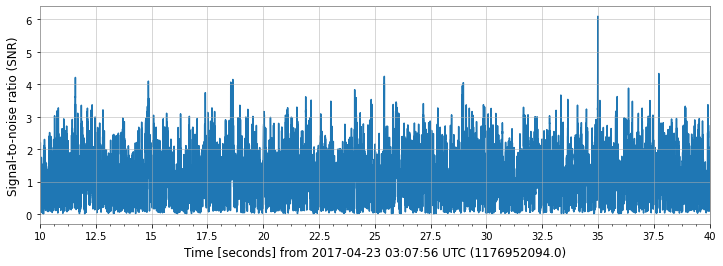
\includegraphics[scale = .33]{laplacian b=2 template 1.png}
\centering
\end{figure} 
In the case of Laplacian noise with $b=2$ (FIG. 12.), the detection result was also accurate (i.e. there is a clear, thin, and distinct peak at time $t=35.0$). However, in this case, the SNR $\rho(t)$ is much lower, reaching only a value of $6.1$. Furthermore, it can be seen that the SNR `noise floor' is also relatively consistent with the Gaussian noise case and the $b=1$ Laplacian noise case, fluctuating around $\rho = 3.0$, though many times reaching $\rho = 4.0$.

In the case of Laplacian noise with scale parameter $b=3$, however, we can make new interesting observations. As shown in FIG. 13., the SNR function $\rho(t)$ has no clear and distinct peaks. Throughout the entire time interval, $\rho(t)$ appears to fluctuate randomly around $\rho = 3$. The function's highest SNR is 4.6, located at time $t=21.7$s, which is clearly inaccurate. However, it is still noteworthy that the SNR value at time $t=35$s is still higher than its surroundings, coming close the maximum value found at time $t=21.7$s.

\begin{figure}[t]
\caption{This figure shows the resulting cropped SNR $\rho(t)$ after a matched filter was applied to recover Template 1 from perfectly Laplacian noise with $b=3$, scaled down by a factor of $10^{-21}$. A signal peak was detected at time $t = 21.7$s with SNR $\rho = 4.6$.}
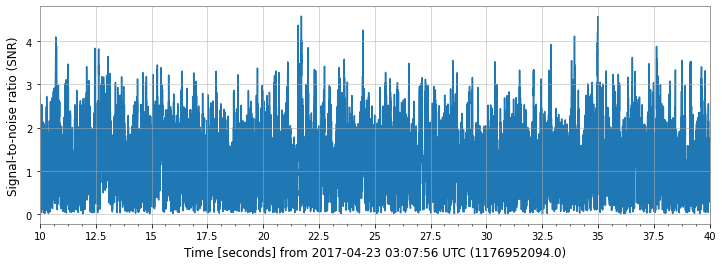
\includegraphics[scale = .33]{laplacian b=3 template 1.png}
\centering
\end{figure}

From the results presented in FIG. 10.,11.,12., and 13., it can be concluded that there is a strong correlation between the kurtosis of the Virgo/LIGO noise distributions and the performance of the matched filter. This observation agrees with the mathematical framework of matched filtering detection algorithm. Although both Laplacian noise (regardless of scale parameter $b$) and Gaussian noise are symmetric about the y-axis, Laplacian noise distributions are much more tail-heavy. This means that when random noise was generated, louder noise was favored. Therefore, it makes mathematical sense that such a probability density distribution would cause a negative effect on the matched filtering detection algorithm.

\begin{figure}[t]
\caption{This figure shows the resulting cropped SNR $\rho(t)$ after a matched filter was applied to recover Template 1 from Glitch 1. A signal peak was detected at time $t = 17.7$s with SNR $\rho = 305.0$.}
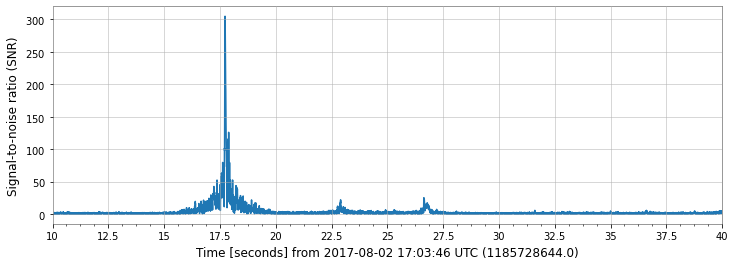
\includegraphics[scale = .33]{glitch loud 69 template 1.png}
\centering
\end{figure}

\begin{figure}[t]
\caption{This figure shows the resulting cropped SNR $\rho(t)$ after a matched filter was applied to recover Template 1 from Glitch 2. A signal peak was detected at time $t = 17.7$s with SNR $\rho = 294.6$.}
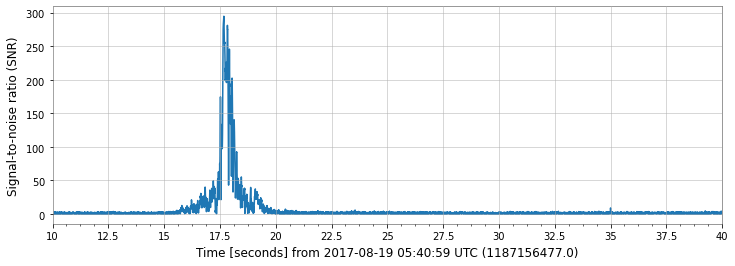
\includegraphics[scale = .33]{glitch loud 02 template 1.png}
\centering
\end{figure}

Shown in Figures 14. and 15. are the detection results for the two \textit{Extremely Loud} glitches (Glitch 1 and Glitch 2). Both of these results share one thing common: They both have an extremely high SNR peak, ranging in the hundreds ($\rho=305.0$ and $\rho=294.6$). It is also worth noticing that these peaks are more triangular / pyramidal in shape – that is, the elevated SNR effects caused by \textit{Extremely Loud} glitches are spread out across multiple frequency bins, and subsequently heavily affect the time-domain data. Moreover, note that in FIG. 14., we can see that Glitch 1 also gave rise to several, lower amplitude false-alarm SNR peaks, in addition the highest peak found at time $t=17.7$s. Similar to the highest peaks, these peaks are more triangular in nature and are of unusually high amplitudes; thus, they can easily be differentiated from real gravitational wave signal.

\begin{figure}[t]
\caption{This figure shows the resulting cropped SNR $\rho(t)$ after a matched filter was applied to recover Template 1 from Glitch 3. A signal peak was detected at time $t = 35.0$s with SNR $\rho = 20.9$.}
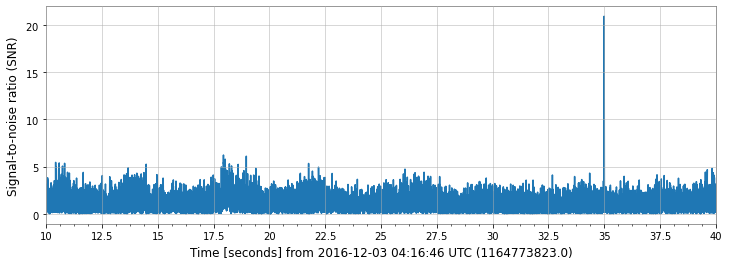
\includegraphics[scale = .33]{glitch 3 template 1.png}
\centering
\end{figure}
\begin{figure}[t]
\caption{This figure shows the resulting cropped SNR $\rho(t)$ after a matched filter was applied to recover Template 1 from Glitch 4. A signal peak was detected at time $t = 35.0$s with SNR $\rho = 21.8$.}
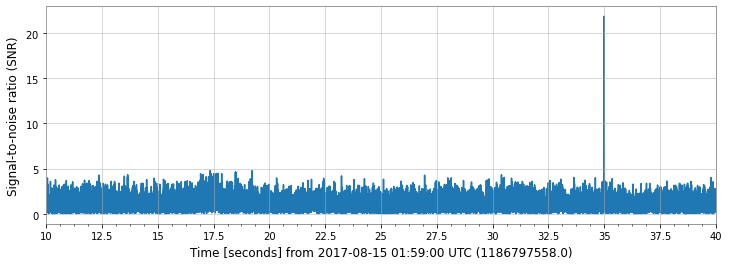
\includegraphics[scale = .33]{glitch 4 template 1.png}
\centering
\end{figure}
\begin{figure}[t]
\caption{This figure shows the resulting cropped SNR $\rho(t)$ after a matched filter was applied to recover Template 1 from Glitch 5. A signal peak was detected at time $t = 35.0$s with SNR $\rho = 20.9$.}
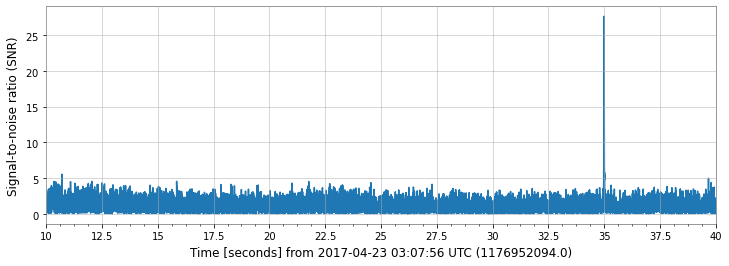
\includegraphics[scale = .33]{glitch 5 template 1.png}
\centering
\end{figure}

Shown in Figures 16. to 18. are the SNR results for the recovery of Template one injected into Glitch 3,4, and 5. Notice that all three of these cases resulted in similar peak SNRs, with all three results reaching a signal-to-noise ratio $\rho$ of around $20$. In addition to that, the SNR `noise floor' is similar all across of three cases, fluctuating at around $\rho\approx 4$. As seen in  \textit{Section IV}, Figures 6., 7., 8., the power distribution of glitches 3,4, and 5 are rather evenly spread out throughout the duration of the glitch. Furthermore, it is worth noting that Template 1 is a relative loud signal – having a peak strain up to $10^{-21}$ orders of magnitude. The effective distance for this template was not too far either, only at the value of $500$ Mpc, which is not that much on an astronomical scale.

\section{Conclusions}
From the data analysis discussed in \textit{Section V} for Template 1, we can conclude that short-duration \textit{Extremely Loud} glitches cause the greatest impact on the performance of the matched filter in gravitational wave detection. Specifically, \textit{Extremely Loud} glitches elevate the signal-to-noise ratio to unusually high levels and can easily mask out real gravitational wave signal. However, the effects of these glitches have distinct characteristics that are worth noting. First, these glitches elevate the signal-to-noise ratio to the extremes, reaching up to the hundreds in magnitude. This characteristic is in clear contrast with real gravitational wave signals, where the resulting SNRs are usually only 2 digits in magnitude. Second, elevated SNR peaks due to \textit{Extremely Loud} glitches have wide bottoms, looking almost pyramidal / triangular like. This is also starkly different from the characteristics of real gravitational wave signals, where the SNR peaks are thin and distinct with no wide bottoms. As a consequent of these observations, we can conclude that if \textit{Extremely Loud} glitches do not coincide with real gravitational wave signals, a data-veto procedure should be incorporated into gravitational wave signal processing. That is, all unusual SNR behavior that mirrors the behavior of \textit{Extremely Loud} glitches should be ignored (or \textit{`vetoed'}). As in the case of the other types of glitches analyzed (\textit{Power Line, Whistle, and Scattered Light}), they pose little to no effects in recovering Template 1's injection into them. Template 1, however, is rather loud. Therefore, this does not reject the possibility that these low-amplitude glitch classifications bear no effects on quieter signals (i.e.\ signals from smaller mass compact binary inspirals). ---- (analysis for template 2, a `quieter' are to be done...)

\section{Summary}
In short, the existence of gravitational waves is a direct consequence of Einstein’s Theory of General Relativity. To detect them, modern science employs an equipment called the Michelson Fabry-Perot Interferometer. In this paper, I discussed three prominent detector sites: LIGO Hanford, LIGO Livingston and Virgo Italy. The detection of gravitational waves is especially challenging and requires extreme precision as wel as sophisticated data analysis tools. One of the most common and efficient data analysis method for the detection of gravitational waves is called matched filtering. Matched filtering performs best when detector noise is perfectly Gaussian and stationary. However, in real life, noise can deviate from these assumptions through the form of transient glitches and different distributions. In such cases, it was shown that the matched filter breaks down when noise distributions are tail-heavy (that is, when they have high kurtoses). Furthermore, the existence of short, \textit{Extremely Loud} glitches can cause exceptionally high SNRs that can easily mask out true gravitational wave signals if the glitch and the signal coincide. (To be continued...)

\section{Some notes for Paper 3 submission...}
This paper only shows my progress so far, in no way does this paper fully reflect the end product for Paper 4. For my final paper, I am intending to complete this paper's analysis for Template 2. I am also hoping to conduct $\chi^2$-significance testing on the SNR results in order to provide some quantitative consideration. Furthermore, I also plan to perform some parameter estimation using the results as well. These procedures will be referenced from the Open Data Workshop tutorials on Day 2. A lot of the time spent in the making of this paper has been devoted to making the PyCBC Python scripts to work well; now that I have this experience, I hope that my work for Paper 4 will progress a little bit more efficiently.

\begin{acknowledgments}
I would like to express my sincerest gratitude to Dr.\ Eric Myers at the State University of New York, New Paltz for guiding me at every step of the way in the making of this paper. Dr. Myers has guided me through my research from the very start, from teaching me the basic background knowledge to helping me with the writing process. I could not be more grateful of Dr.\ Myers' help.

I would also like to thank Michael Zevin (PhD Candidate at Northwestern University), Dr. Peter Shawhan, and other scientists at the LIGO Scientific Collaboration (LSC), and the GravitySpy team for answering many of my technical questions and providing me with the data and documentation that without which, this research would not have been possible. 

This research has made use of data obtained from the Gravitational Wave Open Science Center (\url{https://www.gw-openscience.org}), a service of LIGO Laboratory, the LIGO Scientific Collaboration and the Virgo Collaboration. LIGO is funded by the U.S. National Science Foundation. Virgo is funded by the French Centre National de Recherche Scientifique (CNRS), the Italian Istituto Nazionale della Fisica Nucleare (INFN) and the Dutch Nikhef, with contributions by Polish and Hungarian institutes.
\end{acknowledgments}



\bibliography{citations.bib}% Produces the bibliography via BibTeX.

\end{document}
